%% ------------------------------------------------------------------------- %%
\chapter{Introdução} %Nome do capítulo.
\label{cap:intro} 

O som pode ser definido como a propagação ondulatória e mecânica em um meio elástico
ou como a excitação dos mecanismos auditivos que resultam em sua percepção~\cite{Everest}. No primeiro
caso, estamos tratando de leis puramente físicas. No segundo caso, estamos lidando com um
fenômeno psicofísico. Nesta última abordagem encontramos lugar para a música, que escapa,
portanto, às leis fatídicas dos fenômenos naturais~\cite{Roederer}. A delicada tarefa de capturar estruturas
e artifícios musicais diretamente relacionados às oscilações do som
é exatamente a tarefa proposta por este trabalho. Para isso, entendemos cabível
abordar o som em sua representação digital e dispor os resultados em fórmulas matemáticas e implementações computacionais. 


    \section{Do som ao áudio digital}

Em sua conceituação puramente física, o som é uma onda mecânica logitudinal de pressão e pode se propagar por qualquer meio material.
Embora o corpo humano possa captar sons cujas frequências estão fora da banda compreendida aproximadamente entre $20Hz$ e $20 kHz$, estas são as frequências chamadas audíveis e apreciadas pelo nosso aparelho auditivo.
 Considerada a velocidade do som no ar de $\approx 343.2\,m/s$ em condições usuais,
estes limites correspondem respectivamente aos comprimentos de onda $\frac{343.2}{20} = 17.16\,m$ e $\frac{343.2}{20000}=17.16\,mm$.

A efetiva audição humana destas vibrações consiste em um fenômeno complexo ainda sob intensa pesquisa, involvendo captações pelos ossos, estômago e orelha, além de funções de transferência da cabeça e dorso e processamento pelo sistema nervoso. Existe, no entanto, um órgão dedicado à tarefa de captura destas ondas, ao qual chamamos ouvido e cujo funcionamento decompõe o som em seu espectro senoidal antes de passar o estímulo para o sistema nervoso~\cite{Roederer}. Este papel central das componentes senoidais do som é crucial para os fenomenos musicais, o que pode ser notado tanto na composição de sons de interesse para a música, quanto nas afinações e escalas~\cite{floEsp}.

A representação do som é chamada áudio e usualmente usamos est termo para designar uma representação elétrica do som\footnote{Embora haja esta tendência e tradição de uso, Os termos
som e áudio são, na verdade, usados de forma intercambeável.}. O áudio pode ser proveniente da captura do som por microfones ou da síntese direta. O áudio digital, também chamado som digital, consiste na representação sonora através de protocolos digitais. Alguns destes protocolos são bastante elaborados, em geral visando resultar em quantidades reduzidas de dados para facilitar armazenamento e transferência dos arquivos. Outras representações digitais do som são bastante diretas, consistindo em amostras igualmente espaçadas no tempo e cujas aplitudes individuais são registradas com um mesmo número de bits. Esta representação do som por amostras separadas por intervalos regulares $\lambda_a$ é a forma padrão de representação do com em tempo discreto e é chamada de modulação por código de pulsos (denotada pela sigla PCM do inglêm Pulse Code Modulation).
Um som digital PCM é caracterizado pela frequência de amostragem $f_a=\frac{1}{\lambda_a}$ (também chamada de taxa de amostragem) e profundidade de bit que é o número de bits utilizados para representar cada amostra. Dispomos na figura~\ref{fig:PCM} um esquema gráfico de um áudio PCM.


\begin{figure}[h!]
    \centering
    \caption{Som digital em modulação por código de pulsos (PCM}
        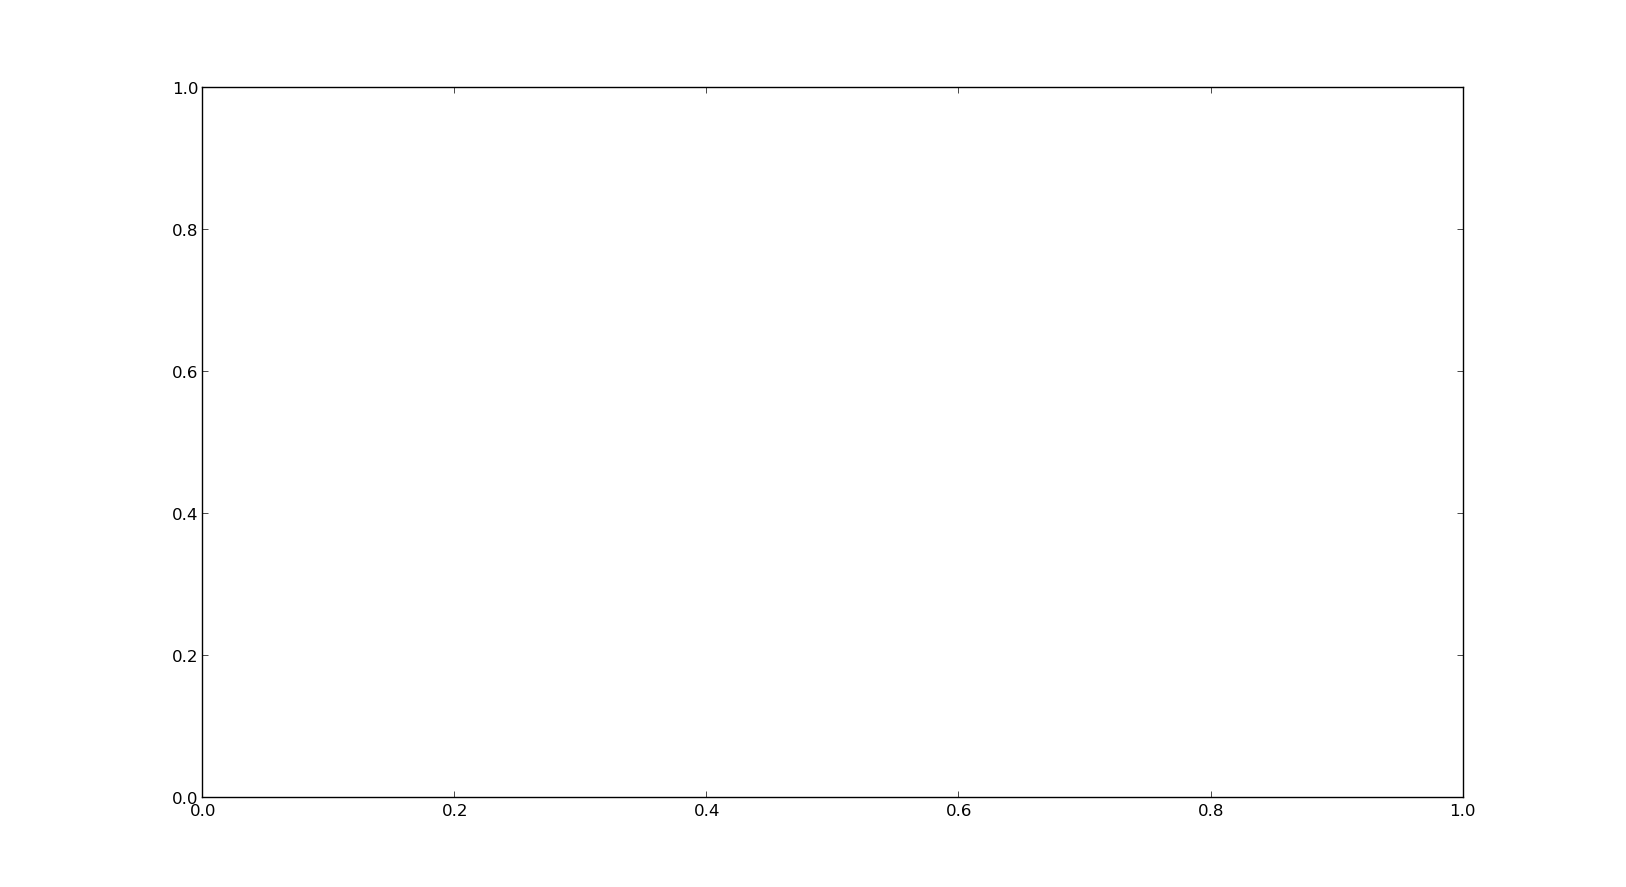
\includegraphics[width=\textwidth]{figuras/foo}
        \label{fig:PCM}
\end{figure}

Nesta representação, é de conhecimento comum pelo teorema de Nyquist que não podemos representar frequências acima da metade da frequência de amostragem. Assim, se buscamos apreender as frequências audíveis, precisamos utilizar uma taxa de amostragem que seja ao menos o dobro da frequência mais alta capturada pelo sistema auditivo $f_a=2.20kHz=40kHz$. Este raciocínio está na base da utilização das frequências de amostragens $f_a=44.1kHz$ e $f_a=48kHz$, ambas utilizadas amplamente e são as taxas de amostragens padrão em \emph{Compact Disks} (CDs) e em sistemas de Rádio e TV, respectivamente.

Do ponto de vista didático, é notável que praticamente todo processamento espectral sonoro seja praticável por somatórios quando tratamos do som discretizado. Estes mesmos procedimentos são obtidos por integrais quando estamos lidando com o som analógico, o que é consideravelmente mais complicado.




    \section{Arte sonora e rudimentos de teoria musical}

A música é comumente definida como a arte manifesta pelos sons e silêncios. Embora esta concepção esteja canonicamente correta, para as concepções usuais, ela está mais associada a uma ideia de arte sonora do que à música propriamente dita. Para um ouvinte comum - e boa parte dos especialistas - a concepção de música exige também a presença de uma métrica rítmica além de organizações de alturas que formem melodias e harmonias (veja sessão~\ref{notasMusica}). De qualquer forma, é importante estabelecer este entendimento e reconhecer que a música do século XX ampliou esta concepção tradicional de música feita por notas que formam rítmos e melodias. Isso ocorreu primeiramente na música de concerto, especialmente nas chamadas correntes eletrônica, concreta e eletroacústica. Já na década de 90 ficou claro que a música popular, especialmente as músicas eletrônicas de dança, tinham por sua vez se desdobrado para abrangir não só sons de altura definida e organizações temporais bem estabelecidas dentro de métricas simples, mas também amálgamas sonoros ruidosos e disposições temporais fluídas e com sobreposições.





    \section{Disponibilização computacional}

    \section{Objetivos}
   \label{sec:objetivos}
